% The finite-element mesh, and the collocation points inside ONE element.
% Second of four composite figures for Lecture 7 (collocation), authored
% 2026-09-08.  This is the canonical mesh cartoon the lecture refers back to,
% so it is deliberately the most explicit of the four.
%
% RELATION TO figures/tikz/collocation-finite-element.tex.  That figure draws a
% GENERIC element with symbolic tau_1 < tau_2 < tau_3 <= 1 and is the picture
% for Sec. "Polynomial representation on one finite element".  This one is the
% MESH: it shows where element i sits inside [t_0, t_f], and then blows that
% element up with the RADAU numbers the lecture actually tells students to type
% (tau_1 = 0.155051, tau_2 = 0.644949, tau_3 = 1; Biegler Table 10.1, p. 292,
% used in Example 10.2, p. 294).  Two figures, two jobs -- do not merge them.
%
% 🔴 tau_3 = 1 IS NOT A DRAWING ERROR.  For Radau the last collocation point
% sits exactly ON the right-hand element boundary, so t_{i3} = t_i and the
% collocation value z_{i3} and the element-endpoint value z_i are the SAME
% point.  The figure draws one dot there and labels it "z_{i3} = z_i", and the
% callout says so in words.  Anyone "fixing" this by pulling tau_3 inside the
% element has broken the picture: it is precisely why Radau collocation makes
% the continuity condition (Eq. 10.15) trivial at that end.
%
% GREYSCALE.  Two hues only -- Okabe-Ito blue #0072B2 (L* = 46) for the state
% polynomial and orange #E69F00 (L* = 70.6) for the collocation apparatus,
% dL* = 24.6.  Every distinction is redundantly encoded: the element-i span is
% marked by a THICKER axis segment as well as a tint, the collocation points
% are FILLED DOTS with dropped rules while the element endpoints are OPEN
% squares, and the zoom is joined by DASHED guide lines.  Nothing is carried by
% colour alone.
%
% TIKZ LIBRARIES.  Base tikz only (plus the >=stealth arrow tip, which both
% preambles provide).  No calc, no patterns, no decorations.pathreplacing --
% the pack preamble and this directory's preamble load different sets, and this
% file stays inside the intersection.

\definecolor{cpblue}{HTML}{0072B2}
\definecolor{cporange}{HTML}{E69F00}

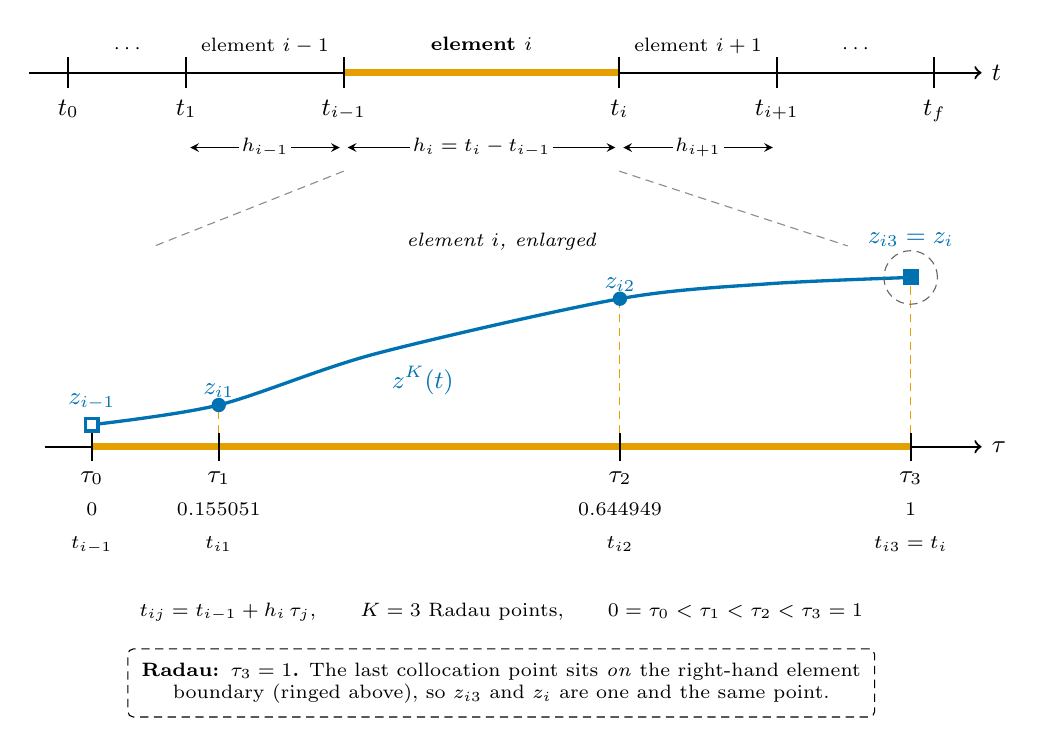
\begin{tikzpicture}[x=1cm, y=1cm, font=\small]

% =========================================================================
% TOP PANEL -- the mesh over the whole horizon.
% Element boundaries: t_0 = 0.5, 2.0, 4.0, 7.5, 9.5, t_f = 11.5.
% Element i is [4.0, 7.5]; it is drawn wider than its neighbours because it is
% the one that gets blown up below.
% =========================================================================

% The horizon, with element i drawn very thick so the zoom target is legible
% without relying on the tint.
\draw[->, thick] (0,0) -- (12.1,0) node[right] {$t$};
\draw[cporange, line width=2.4pt] (4.0,0) -- (7.5,0);

\foreach \x in {0.5, 2.0, 4.0, 7.5, 9.5, 11.5}
  \draw[thick] (\x,-0.2) -- (\x,0.2);

\node[below] at (0.5,-0.22)  {$t_0$};
\node[below] at (2.0,-0.22)  {$t_{1}$};
\node[below] at (4.0,-0.22)  {$t_{i-1}$};
\node[below] at (7.5,-0.22)  {$t_{i}$};
\node[below] at (9.5,-0.22)  {$t_{i+1}$};
\node[below] at (11.5,-0.22) {$t_f$};

% Element names above the axis.
\node[above, font=\scriptsize] at (3.0,0.12)  {element $i-1$};
\node[above, font=\scriptsize] at (5.75,0.16) {\textbf{element $i$}};
\node[above, font=\scriptsize] at (8.5,0.12)  {element $i+1$};
\node[above, font=\scriptsize] at (1.25,0.12) {$\cdots$};
\node[above, font=\scriptsize] at (10.5,0.12) {$\cdots$};

% Element lengths.
\draw[<->, >=stealth] (2.05,-0.95) -- (3.95,-0.95);
\node[font=\scriptsize, fill=white, inner sep=1pt] at (3.0,-0.95) {$h_{i-1}$};
\draw[<->, >=stealth] (4.05,-0.95) -- (7.45,-0.95);
\node[font=\scriptsize, fill=white, inner sep=1pt] at (5.75,-0.95)
  {$h_i = t_i - t_{i-1}$};
\draw[<->, >=stealth] (7.55,-0.95) -- (9.45,-0.95);
\node[font=\scriptsize, fill=white, inner sep=1pt] at (8.5,-0.95) {$h_{i+1}$};

% =========================================================================
% ZOOM -- dashed guides fanning out from element i towards the blow-up panel.
% They stop SHORT of the panel on purpose: run them all the way to the panel
% corners and they cut straight through the state polynomial and the
% "z_{i3} = z_i" label.  Stopping at y = -2.2 makes the same point and leaves
% the drawing clean.
% =========================================================================
\draw[black!45, densely dashed] (4.0,-1.25) -- (1.6,-2.2);
\draw[black!45, densely dashed] (7.5,-1.25) -- (10.4,-2.2);
\node[font=\scriptsize\itshape] at (6.0,-2.15) {element $i$, enlarged};

% =========================================================================
% BOTTOM PANEL -- element i, in normalized time tau in [0,1].
% tau = 0 maps to x = 0.8 and tau = 1 maps to x = 11.2, so
%   x(tau) = 0.8 + 10.4 * tau.
%   tau_1 = 0.155051 -> x = 2.4125
%   tau_2 = 0.644949 -> x = 7.5075
%   tau_3 = 1        -> x = 11.2      <-- ON the boundary.  Deliberate.
% Baseline of this panel: y = -4.75.
% =========================================================================

% The state polynomial across the element.
\draw[cpblue, very thick]
  plot[smooth] coordinates {(0.8,-4.47) (2.4125,-4.22) (4.4,-3.57)
    (7.5075,-2.87) (9.4,-2.68) (11.2,-2.60)};
\node[cpblue, below right, font=\small, inner sep=3pt] at (4.5,-3.62)
  {$z^K(t)$};

% Element endpoints: OPEN SQUARES, so they are told from the collocation dots
% by shape and not only by colour.
\draw[cpblue, very thick, fill=white] (0.72,-4.55) rectangle ++(0.16,0.16);
\node[cpblue, above, inner sep=3pt] at (0.8,-4.39) {$z_{i-1}$};

% Collocation points 1 and 2: filled dots with a dropped rule to the axis.
\foreach \x/\y/\lab in {2.4125/-4.22/{z_{i1}}, 7.5075/-2.87/{z_{i2}}} {
  \draw[cporange, densely dashed] (\x,-4.75) -- (\x,\y);
  \fill[cpblue] (\x,\y) circle (2.6pt);
  \node[cpblue, above, inner sep=2.5pt] at (\x,\y) {$\lab$};
}

% Collocation point 3 == the element endpoint.  ONE dot, drawn as a filled dot
% INSIDE an open square, because it is genuinely both things at once, and
% ringed so the eye goes there before it reaches the note at the bottom.
\draw[cporange, densely dashed] (11.2,-4.75) -- (11.2,-2.60);
\draw[cpblue, very thick, fill=white] (11.12,-2.68) rectangle ++(0.16,0.16);
\fill[cpblue] (11.2,-2.60) circle (2.6pt);
\draw[black!60, densely dashed] (11.2,-2.60) circle (0.34);
\node[cpblue, above, inner sep=11pt] at (11.2,-2.60) {$z_{i3} = z_i$};

% ------------------------------------------------------------- the tau axis
\draw[->, thick] (0.2,-4.75) -- (12.1,-4.75) node[right] {$\tau$};
\draw[cporange, line width=2.4pt] (0.8,-4.75) -- (11.2,-4.75);
\foreach \x in {0.8, 2.4125, 7.5075, 11.2}
  \draw[thick] (\x,-4.93) -- (\x,-4.57);

% Three stacked labels per point: the symbol, the Radau number, the physical
% time.  t_{ij} = t_{i-1} + h_i tau_j, printed under the panel.
\node[below, align=center, inner sep=3pt] at (0.8,-4.95)
  {$\tau_0$\\[1pt]{\scriptsize $0$}\\[1pt]{\scriptsize $t_{i-1}$}};
\node[below, align=center, inner sep=3pt] at (2.4125,-4.95)
  {$\tau_1$\\[1pt]{\scriptsize $0.155051$}\\[1pt]{\scriptsize $t_{i1}$}};
\node[below, align=center, inner sep=3pt] at (7.5075,-4.95)
  {$\tau_2$\\[1pt]{\scriptsize $0.644949$}\\[1pt]{\scriptsize $t_{i2}$}};
\node[below, align=center, inner sep=3pt] at (11.2,-4.95)
  {$\tau_3$\\[1pt]{\scriptsize $1$}\\[1pt]{\scriptsize $t_{i3} = t_i$}};

% ------------------------------------------------------------- the callouts
\node[align=center, font=\scriptsize] at (6.0,-6.85)
  {$t_{ij} = t_{i-1} + h_i\,\tau_j$,\qquad
   $K = 3$ Radau points,\qquad $0 = \tau_0 < \tau_1 < \tau_2 < \tau_3 = 1$};

% A boxed sentence rather than a boxed callout with a leader: any arrow drawn
% to the ringed point crosses either the tau labels or the tau axis, and the
% ring plus the named symbols carry the reference perfectly well.
\node[draw, densely dashed, rounded corners=2pt, align=center,
      font=\scriptsize, inner sep=5pt, fill=white] at (6.0,-7.75)
  {\textbf{Radau: $\tau_3 = 1$.} The last collocation point sits \emph{on} the
   right-hand element\\ boundary (ringed above), so $z_{i3}$ and $z_i$ are one
   and the same point.};

\end{tikzpicture}
